\documentclass[11pt]{article}

\input{preambulo.tex}

\usepackage{booktabs}
\usepackage{multirow}
\usepackage{listings}
\usepackage{xcolor}
\usepackage{subcaption}
\usepackage[table]{xcolor}
\usepackage{titlesec}

\colorlet{maincolor}{Violet}

% Definición de colores pastel y modernos
\definecolor{backcolour}{rgb}{0.96,0.96,0.96}
\definecolor{codegreen}{rgb}{0.13,0.55,0.13}
\definecolor{codegray}{rgb}{0.5,0.5,0.5}
\definecolor{codepurple}{rgb}{0.58,0,0.82}
\definecolor{codeblue}{rgb}{0.0,0.0,0.8}

% Configuración del estilo moderno
\lstdefinestyle{modern}{
    backgroundcolor=\color{backcolour},   
    commentstyle=\color{codegreen}\itshape,
    keywordstyle=\color{codeblue}\bfseries,
    numberstyle=\tiny\color{codegray},
    stringstyle=\color{codepurple},
    basicstyle=\ttfamily\scriptsize,
    breakatwhitespace=false,         
    breaklines=true,                 
    captionpos=b,                    
    keepspaces=true,                 
    numbers=left,                    
    numbersep=10pt,                  
    showspaces=false,                
    showstringspaces=false,
    showtabs=false,                  
    tabsize=4,
    frame=single,                    % Marco simple alrededor del código
    rulecolor=\color{lightgray},     % Color del marco
    xleftmargin=15pt,                % Margen para que los números no se peguen
    literate={á}{{\'a}}1 {é}{{\'e}}1 {í}{{\'i}}1 {ó}{{\'o}}1 {ú}{{\'u}}1
             {Á}{{\'A}}1 {É}{{\'E}}1 {Í}{{\'I}}1 {Ó}{{\'O}}1 {Ú}{{\'U}}1
             {ñ}{{\~n}}1 {Ñ}{{\~N}}1
}

% Aplicar el estilo por defecto a todos los bloques de código
\lstset{style=modern}

% --- CONFIGURACIÓN DE SECCIONES ---

% Formato para \section
% Sintaxis: \titleformat{\comando}{formato}{etiqueta}{separación}{antes_del_texto}
\titleformat{\section}
  {\color{maincolor}\large\bfseries} % Color, fuente, tamaño y estilo
  {\thesection.} % Muestra el número de sección (ej. 1, 2...)
  {0.5em} % Espacio entre el número y el texto del título
  {} % Código adicional antes del texto del título

% Formato para \subsection
\titleformat{\subsection}
  {\color{maincolor}\large\bfseries} % Color vino, tamaño grande, cursiva
  {\thesubsection}
  {0.5em}
  {}

\title{}
\author{Jesús Muñoz Velasco}
\date{Curso 2025-2026}

\begin{document}

{\Large \bfseries \centering \color{maincolor} Práctica 1: Desarrollo de agentes basado en técnicas de búsqueda heurística dentro del entorno GVGAI}

\vspace{0.25cm}
{\large \bfseries \color{maincolor} Autor: Jesús Muñoz Velasco}

\section{Métricas obtenidas y análisis de resultados}
Tras ejecutar cada algoritmo en cada uno de los mapas especificados por el guion se han obtenido los siguientes resultados:

\begin{table}[H]
    \centering
    \label{tab:metricas_resultados_DFS}
    \arrayrulecolor{Violet!25}
    \begin{tabular}{|c | c | c | c | c |}
        \hline
        \rowcolor{Violet}
        \color{white} Mapa & \color{white} Nº Acciones & \color{white} Nodos Expandidos & \color{white} Profundidad Máxima & \color{white} t(ms)\\
        0 & 66 & 157 & 66 & 12 \\
        5 & 217 & 272 & 217 & 91 \\
        6 & 139 & 166 & 139 & 23 \\
        \hline
    \end{tabular}%
    \caption{Resultados de ejecución del Algoritmo de Búsqueda en profundidad}
\end{table}

\begin{table}[H]
    \centering
    \label{tab:metricas_resultados_Astar}
    \arrayrulecolor{Violet!25}
    \begin{tabular}{| c | c | c | c | c | c |}
        \hline
        \rowcolor{Violet} \color{white} Mapa & \color{white} Nº Acciones & \color{white} Nodos Abiertos & \color{white} Nodos Cerrados & \color{white} Nodos Expandidos & \color{white} t(ms)\\
        0 & 48 & 209 & 5 & 209 & 4\\
        5 & 188 & 2621 & 51 & 2621 & 81\\
        6 & 78 & 1980 & 100 & 1980 & 18\\
        \hline
    \end{tabular}%
    \caption{Resultados de ejecución del Algoritmo A*}
\end{table}

\begin{table}[H]
    \centering
    \label{tab:metricas_resultados_RTAStar}
    \arrayrulecolor{Violet!25}
    \begin{tabular}{| c | c | c | c | c |}
        \hline
        \rowcolor{Violet} \color{white} Mapa & \color{white} Nº Acciones & \color{white} Nodos Expandidos  & \color{white} t(ms) & \color{white} Encuentra Salida\\
        0 & 38 & 38 & 2 & No \\
        5 & 1941 & 1941 & 728 & Sí \\
        6 & 403 & 403 & 70 & Sí \\
        \hline
    \end{tabular}%
    \caption{Resultados de ejecución del Algoritmo RTA*}
\end{table}

\begin{table}[H]
    \centering
    \label{tab:metricas_resultados_LRTAStarK}
    \arrayrulecolor{Violet!25}
    \begin{tabular}{| c | c | c | c | c | c | c |}
        \hline
        \rowcolor{Violet} \color{white} Mapa & \color{white} Nº Acciones & \color{white} Nodos Expandidos & \color{white} Actualizaciones $h$ & \color{white} t(ms)& \color{white} Encuentra Salida\\
        0 & 38 & 38 & 15 & 3 & No\\
        5 & 3203 & 3203 & 3395 & 1201 & Sí \\
        6 & 343 & 343 & 363 & 54 & Sí \\
        \hline
    \end{tabular}%
    \caption{Resultados de ejecución del Algoritmo LRTA*(k) para $k=5$}
\end{table}

Con estas medidas podemos hacer una comparativa de algoritmos:
\subsection{Búsqueda en Profundidad}
Una clara ventaja de este algoritmo es que expande relativamente pocos nodos en comparación con A*, pero los caminos que encuentra no son óptimos. Al explorar una sola rama puede encontrar la solución rápidamente en mapas simples además de ser bastante óptimo en memoria. Aun así tiene la clara desventaja de no ser óptimo ni completo (no encuentra la solución óptima, como se puede ver al compararlo con A*). Puede ser muy útil en casos donde el uso de memoria debe ser mínimo y no se busque encontrar la solución óptima sino una aceptable en entornos conocidos y estáticos (sobre todo en mapas bastante grandes, donde otros algoritmos como A* tardarían demasiado).

\subsection{A*}
Es el único algoritmo que encuentra la ruta óptima y esta es su principal ventaja (es óptimo y completo al tener una heurística admisible). Sin embargo, en mapas muy grandes el uso de memoria puede dispararse (es el que más nodos expande de media) y por tanto también el tiempo de cálculo tenderá a aumentar en estos casos. Es por esto que es el mejor cuando se disponga de gran capacidad de memoria y de cómputo, y cuando se priorice encontrar la solución óptima en entornos conocidos y estáticos. En caso de problemas simples como el que estamos trabajando es sin duda la mejor opción con diferencia (ofrece los mejores tiempos y asegura encontrar siempre la solución óptima si existe).

\subsection{Real-Time A* (RTA*)}
Uno de los problemas que encontramos en este algoritmo es que no siempre encuentra la solución (en ejecuciones que no aparecen en las tablas vemos que para los niveles del 0 al 4 no encuentra la salida). Sin embargo, expande en general menos nodos que LRTA*(k) (algoritmo con el que comparamos este) y en cuanto a resultados solo podemos decir que ha resultado bastante mejor en el mapa más grande (el 5) aunque ligeramente peor en el nivel 6. Aparece también la desventaja de no ser óptimo ni completo. Su principal ventaja frente a los dos algoritmos anteriores es que no necesita conocer el mapa a priori por lo que en mapas desconocidos puede ser la mejor opción (sobre todo en mapas grandes) y que toma decisiones rápidas en cada caso (puede reaccionar a cambios del entorno si fuera necesario).

\subsection{Learning Real-Time A* (LRTA*(k))}
Sin duda la mayor ventaja de este algoritmo con respecto al anterior es la capacidad de aprender (virtud que no se explota al ejecutarlo una única vez). Si lo ejecutáramos varias veces veríamos como poco a poco iría convergiendo a la solución óptima gracias a actualizar las heurísticas del mapa virtual. Su principal desventaja es que le cuesta resolver mapas complejos de primeras, ofreciendo el peor resultado con mucha diferencia en el mapa 5 (3203 acciones frente a las 188 que ejecuta A*) aunque como ya se ha comentado, en sucesivas ejecuciones mejoraría notablemente este resultado (incluso con pequeñas variaciones del mapa, ya que no deja de ser un algoritmo de tiempo real). Es por esto que su objetivo principal es operar de forma repetitiva sobre un entorno desconocido pero ligeramente estático (ya que sino el aprendizaje no serviría para nada).

\subsection{Conclusiones}
Para el problema que estamos trabajando (mapa estático y previamente conocido) el mejor algoritmo en todos los aspectos es A* por los motivos que ya se han comentado aunque si el problema dejase de ser estático (como el modo competición) quizás deberíamos recurrir a un algoritmo más basado en LRTA*(k) gracias a su capacidad de aprender y reaccionar al entorno.

\section{Búsqueda bidireccional}
\subsection{Representación del estado}
Para la representación del estado del juego tendría en cuenta los siguientes parámetros en la estructura de un nodo:

\begin{lstlisting}[language=C++]
// Posición del avatar en el mapa
int pos_x;
int pos_y;

int capa;               // Capa actual (-1: sin capa, 0: capa roja, 1: capa azul)
long capa_roja_bitmask;  // Cada bit es una capa roja en el mapa 
                        // (0: no recogida, 1: recogida) 
long capa_azul_bitmask;  // Cada bit es una capa azul en el mapa 
                        // (0: no recogida, 1: recogida)
\end{lstlisting}
Para que esto funcione (la máscara de bits en concreto), el agente tendría que tener un mapa hash como el siguiente:
\begin{lstlisting}[language=C++]
private HashMap<Position, Integer> itemToIndex;
\end{lstlisting}
que le permita traducir posiciones del mapa a posiciones de la máscara de bits (misma estrategia que uso en la práctica para saber las monedas, llaves y catapultas recogidas y restantes en el mapa).

\subsection{Problemáticas de la búsqueda bidireccional}
El primer problema que vemos en la búsqueda bidireccional es que no hay un único estado objetivo, entendiendo el estado como se ha descrito previamente, ya que podría llegar a la meta con una capa azul, una roja o sin capa y haber recogido un número variable de capas de cada tipo durante el proceso (bitmaks distintos). Esto plantea que no haya un único ``nodo inicial'' cuando se comienza la búsqueda desde el nodo objetivo (en teoría vimos que esto se podía solucionar creando un nuevo nodo objetivo y uniéndolo a todos estos, pero en este caso hay demasiadas combinaciones posibles, en especial si hay varias capas en el mapa).\\

Otro problema claro es que al avanzar, recoger una capa destruye la anterior y elimina la nueva del mapa, pero hacia atrás esto funciona justo al revés: el agente tendría que "soltar" la capa en el mapa y adivinar qué capa llevaba puesta antes. Esto plantea el mismo problema que antes, ya que habría demasiadas posibilidades acerca de dónde soltar la capa y cuál ponerse, y se ramificaría mucho el árbol de estados.

\subsection{Diferencias en representación \textit{forward} y \textit{backward}}
La representación del estado que se ha descrito anteriormente parece funcionar muy bien en la estrategia \textit{forward} ya que es determinista (un único estado inicial y un único estado cada vez que se mueve). Sin embargo, por los problemas de ramificación que ya se han comentado parece no ser la mejor representación para la estrategia \textit{backward}. Una posibilidad sería relajar las condiciones (no hacer tan estático el estado) de forma que no intente ``adivinar'' de dónde viene si no lo puede saber (como intentar adivinar dónde soltar una capa o qué capa llevaba antes) sino dejarlo de forma indeterminada (aunque esto complicaría la validación de acciones como si puedo atravesar un muro rojo, donde se podría asumir que llevaba puesta la capa roja, con la complicación de que no sé de dónde he cogido esta capa).

\subsection{Choque de fronteras}
Si se han conseguido solucionar todos los problemas de representación que se han mencionado antes podríamos llegar al punto en el que se encontrasen las fronteras, y en este caso solo se asumiría que se ha encontrado la solución si ambas coinciden completamente en el estado completo (con la representación inicial que se ha hecho). Si esto no fuese así no se puede asumir que eso es una solución (ya que a lo mejor \textit{forward} no lleva capa y \textit{backward} lleva una capa roja que asume que va a necesitar para atravesar cierto muro). 

\subsection{Optimalidad de la solución}
Técnicamente este algoritmo, si se consiguen solucionar todos los problemas que ya se han comentado sí que debería ser óptimo, aunque no sería la mejor estrategia para este caso, ya que como se ha comentado, el factor de ramificación en \textit{backward} es demasiado alto y puede no ser práctico de manejar. Para mí el mejor algoritmo en este caso es A* con una heurística admisible como la distancia Manhattan, ya que se conoce todo el mapa a priori y el cambio de estado de un nodo es determinista (con el significado que se ha explicado antes). Sería un caso muy parecido al de la práctica trabajada pero con el estado representado anteriormente.

\section{Análisis de LRTA*(k)}

\subsection{Comienzo en una posición diferente}
Si el agente comienza en una posición diferente hay dos posibles situaciones:
\begin{itemize}
    \item \textbf{El agente comienza en una zona explorada.} En este caso el agente aprovecharía al máximo los beneficios de este algoritmo, ya que la heurística (aprendizaje) iría guiando al agente hacia la salida, en especial si ya se ha ejecutado varias veces (cuanto más se haya hecho más rápido debería de encontrar la solución). 
    \item \textbf{El agente comienza en una zona desconocida.} Este caso es ligeramente peor que el anterior, pero aun así no desaprovecha las ventajas de LRTA*(k). Comenzaría explorando la zona, actualizando $h$ en esas posiciones nuevas hasta llegar a una zona explorada o hasta encontrar un camino a la salida. En cualquiera de estos casos, aunque no sería lo más óptimo para superar el nivel, sí que beneficiaría mucho más el aprendizaje, aumentando la zona explorada y beneficiando que se encuentre una mejor solución desde cualquier posible posición inicial en posteriores ejecuciones. 
\end{itemize}

\subsection{El estado objetivo es diferente}
Si mantenemos el aprendizaje pero cambiamos el objetivo (por ejemplo la posición del portal de salida) sería muy perjudicial de primeras, ya que el agente ha aprendido a moverse hacia el objetivo anterior y tendría que ejecutarse muchas veces para compensar de alguna forma el aprendizaje anterior con el nuevo y en cualquier caso, en lugar de aprovechar el aprendizaje previo, este le perjudicaría.\\

Otro problema que esto presenta es la pérdida de admisibilidad (ya que la heurística anterior era admisible para el objetivo anterior pero no se garantiza que lo sea para este). Un nodo que esté ahora ``cerca'' del nodo objetivo puede que estuviera antes ``lejos'' de lo que era el objetivo, sobreestimando el coste esperado.\\

Sin ninguna duda lo mejor que se puede hacer es ``resetear'' la heurística (aprendizaje) si el objetivo cambia, ya que solo perjudica el hecho de mantenerla.

\section{Pérdida de solución única}
En esta sección se nos pide eliminar un elemento del estado del nodo (que no sea la posición) y que pueda dar lugar a dos soluciones distintas. En este caso vamos a eliminar toda la presencia acerca de las llaves (\verb|keys| y \verb|keys_bitmask|) y vamos a considerar el caso más simple, que es el siguiente mapa:

\begin{center}
    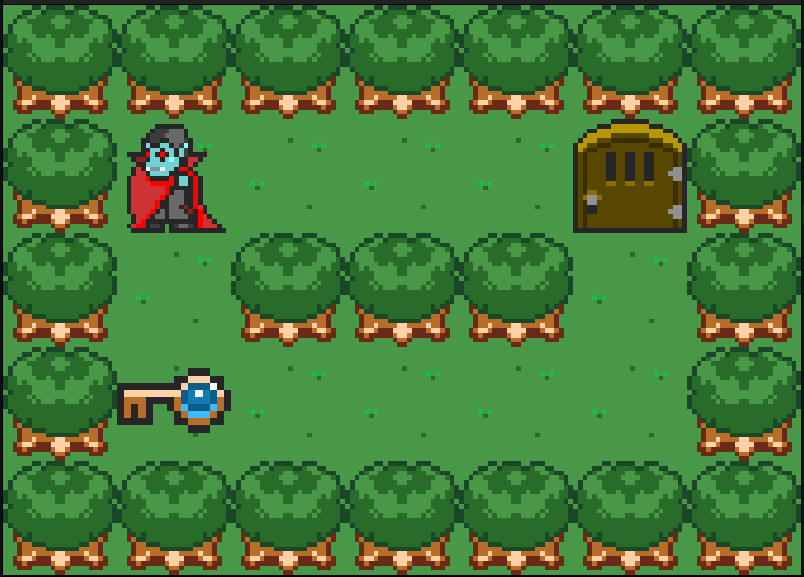
\includegraphics[width=7cm]{img/captura_mapaejercicio4.png}
\end{center}

Al no considerar la llave, el agente podría suponer que puede salir por la puerta e iría el línea recta dando lugar a la siguiente solución:

\begin{center}
    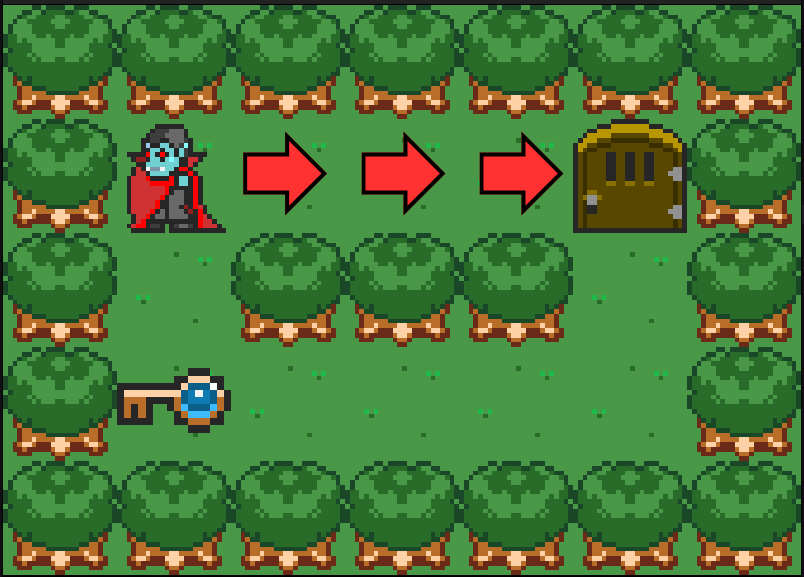
\includegraphics[width=7cm]{img/captura_mapaejercicio4_sol1.png}
\end{center}

Que claramente no sería una solución válida. Otra posible solución (la válida y que coincidiría con la única si considerásemos las llaves en el estado) sería:

\begin{center}
    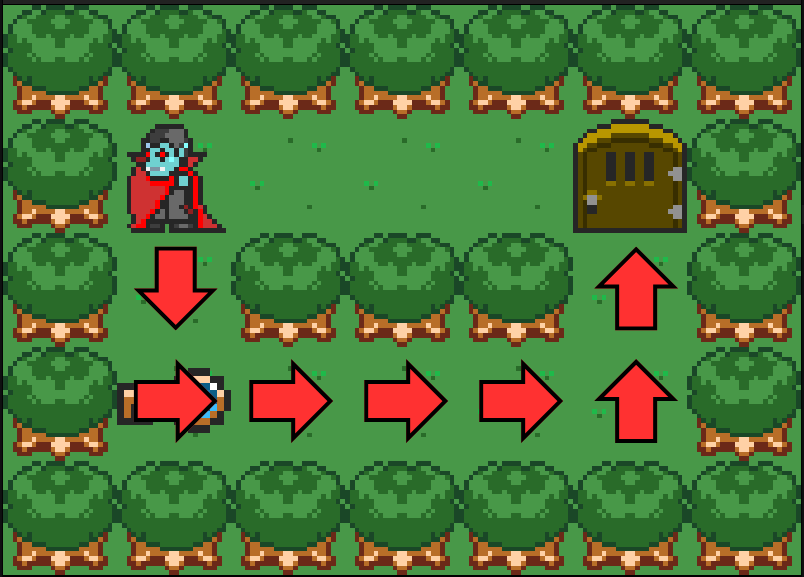
\includegraphics[width=7cm]{img/captura_mapaejercicio4_sol2.png}
\end{center}

Esto se debe a que al eliminar toda la información sobre si un agente posee o no la llave este no puede hacer comprobaciones acerca de si la solución es válida basándose en la posesión de esta, debido a que la única herramienta que tendría para saber si es solución es haber llegado a la posición del portal. Es por esto que es muy importante representar el estado de forma completa (aunque en este caso parece algo tan trivial hay casos en los que no lo es tanto).

\end{document}
